\section*{PHẦN I: NỘI DUNG THỰC TẬP}
\addcontentsline{toc}{section}{\numberline{} PHẦN I: NỘI DUNG THỰC TẬP}

\subsection*{1. Mục đích thực tập}
\addcontentsline{toc}{subsection}{\numberline{} 1. Mục đích thực tập} 
Thông qua việc thực tập ngoài trường của sinh viên, môn học cung cấp trải
nghiệm về môi trường làm việc thực tế, giúp sinh viên nhận thức về các vấn đề đạo đức
nghề nghiệp, tăng cường khả năng làm việc nhóm, cũng như khả năng giao tiếp.
Môn học tạo điều kiện cho người học áp dụng các kỹ thuật, kỹ năng, và công cụ
kỹ thuật hiện đại để giải quyết các vấn đề thiết kế đương đại của ngành Kỹ thuật Điện.
\\

\subsection*{2. Thời gian thực tập}
\addcontentsline{toc}{subsection}{\numberline{} 2. Thời gian thực tập} 

\begin{table}[H]
	\centering
	\begin{tabular}{|l|l|}
		\hline
		\multicolumn{1}{|c|}{\textbf{Thời gian}} & \multicolumn{1}{c|}{\textbf{Công việc thực tập}}                                                                            \\ \hline
		\textbf{Tuần 1: 12/6/2024 – 18/6/2024}    & \multirow{2}{*}{\begin{tabular}[c]{@{}l@{}}Tìm hiểu và sử dụng Gateway Industrial 4G \\ Edge Ro.\end{tabular}}              \\ \cline{1-1}
		\textbf{Tuần 2: 19/6/2024 – 25/6/2024}    &                                                                                                                             \\ \hline
		\textbf{Tuần 3: 26/6/2024 – 2/7/2024}     & Phát triển hệ thống giám sát cường độ sáng.                                                                                       \\ \hline
		\textbf{Tuần 4: 3/7/2024 – 9/7/2024}      & \begin{tabular}[c]{@{}l@{}}Kiểm tra hoạt động ADC trên hai dòng chip\\ AVR và STM32.\end{tabular}                           \\ \hline
		\textbf{Tuần 5: 10/7/2024 – 16/7/2024}    & \multirow{3}{*}{\begin{tabular}[c]{@{}l@{}}Nghiên cứu và phát triển USB Mass Strorage \\ bằng ESP32 và STM32.\end{tabular}} \\ \cline{1-1}
		\textbf{Tuần 6: 17/7/2024 – 23/7/2024}    &                                                                                                                             \\ \cline{1-1}
		\textbf{Tuần 7: 17/7/2024 – 23/7/2024}    &                                                                                                                             \\ \hline
		\textbf{Tuần 8: 23/7/2024 – 31/7/2024}    & \begin{tabular}[c]{@{}l@{}}Viết tài liệu tham khảo về FATFs và cách sử \\ dụng FATFs.\end{tabular}                          \\ \hline
	\end{tabular}
	\caption{Lịch trình thực tập}
\end{table}

Thời gian thực tập: 3/6/2024 - 30/8/2024.

\subsection*{3. Địa điểm thực tập}
\addcontentsline{toc}{subsection}{\numberline{} 3. Địa điểm thực tập} 

Địa điểm thực tập: Phòng thí nghiệm 209B3.

\subsection*{4. Nội dung thực tập}
\addcontentsline{toc}{subsection}{\numberline{} 4. Nội dung thực tập} 

\subsubsection*{4.1. Tìm hiểu và sử dụng Gateway Industrial 4G Edge Ro}
\addcontentsline{toc}{subsection}{\numberline{} 4.1. Tìm hiểu và sử dụng Gateway Industrial 4G Edge Ro} 

\begin{figure}[H]
	\centering
	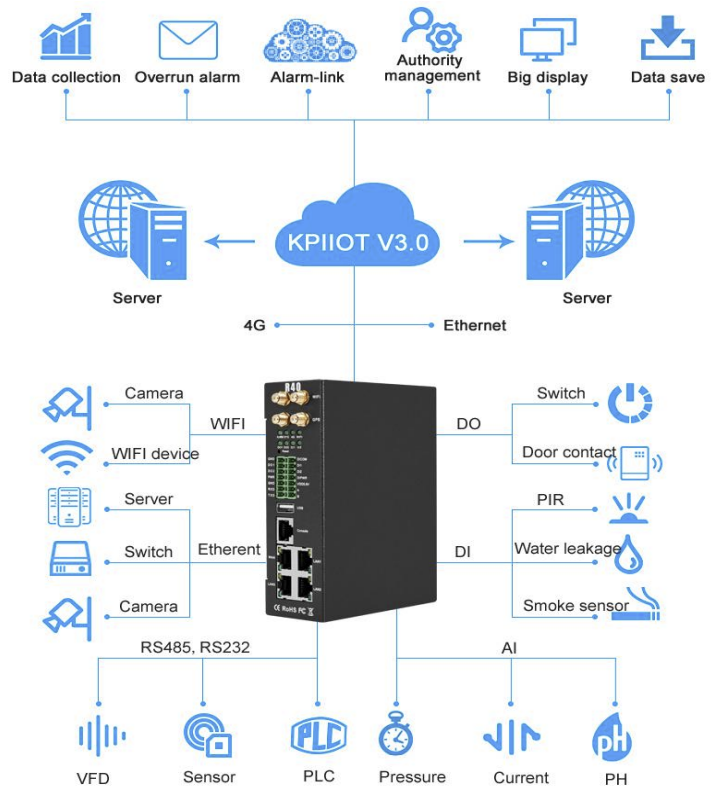
\includegraphics[scale=0.8]{Image/Content_1/Gateway.png}
	\caption{Industrial 4G Edge Ro}
\end{figure}

R40 là bộ định tuyến biên công nghiệp, tương thích với mạng 4G/3.5G/3G/2.5G, hàng đầu
cấu hình, liên kết VPN, bảo vệ công nghiệp, nhiệt độ rộng, thiết kế điện áp rộng, dễ cài đặt
tốc độ cao, ổn định. Mạng truyền dẫn không dây sử dụng mạng LTE công cộng để cung cấp cho người dùng
với khả năng truyền dữ liệu đường dài không dây, có thể được sử dụng trong nhiều ứng dụng công nghiệp.
Đây là thiết bị đầu cuối Internet of Things đa chức năng cấp công nghiệp hỗ trợ nguồn POE
cung cấp, đi kèm đầu vào và đầu ra IO, có 2 cổng nối tiếp, hỗ trợ truyền dẫn trong suốt, giao thức Modbus Master để mở rộng IO và kết nối PLC và các thiết bị khác.\\
Thiết bị này sử dụng SIM kép thiết kế dự phòng thẻ để đảm bảo truyền dữ liệu ổn định và đáng tin cậy, hỗ trợ giao thức MQTT và Giao thức Modbus, giao thức SNMP và tương thích với hầu hết các giao thức PLC, đơn giản hóa rất nhiều chi phí xây dựng hệ thống dây điện tại chỗ và giảm chi phí vận hành và bảo trì. 
\\

\subsubsection*{4.2. Phát triển hệ thống giám sát độ sáng}
\addcontentsline{toc}{subsection}{\numberline{} 3.2. Phát triển hệ thống giám sát độ sáng} 

Sử dụng cảm biến:

\begin{figure}[H]
	\centering
	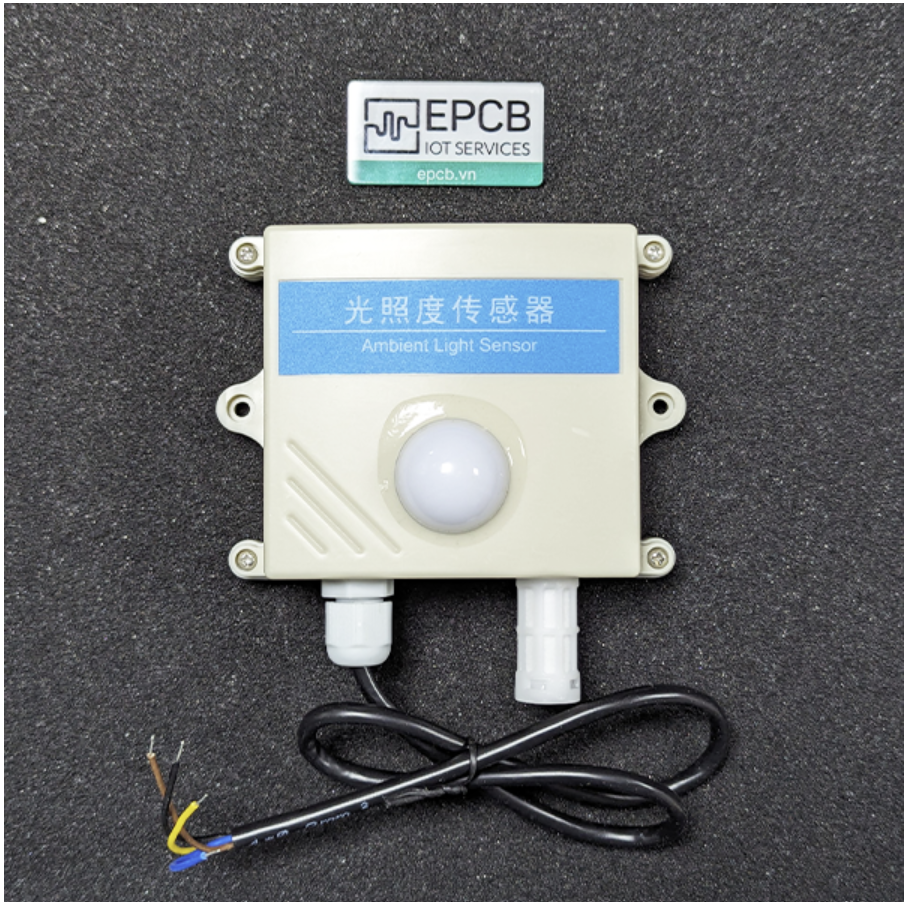
\includegraphics[scale=0.8]{Image/Content_1/Sensor.png}
	\caption{Cảm biến ánh sáng công nghiệp ES-ALS-01}
\end{figure}

Cảm biến ánh sáng công nghiệp ES-ALS-01 là dòng cảm biến đo cường độ sáng cho kết quả chính xác, ổn định và đáng tin cậy. Ngõ ra RS485 Modbus RTU giúp dễ dàng kết nối đến bất cứ hệ thống điều khiển và giám sát nào (MCU, HMI, PLC, PC...). Phù hợp các ứng dụng: Nhà kính nông nghiệp, Thí nghiệm, Mưa tuyết ngoài trời, Chiếu sáng nhà máy,...
\\

\begin{table}[H]
	\centering
	\begin{tabular}{|l|l|} 
		\hline
		{\textbf{Cấp nguồn}}                     & { \textbf{12-24VDC}}    \\ 
		\hline
		{\textbf{Cổng tín hiệu}}                 & { RS485 (Modbus RTU)}   \\
		\hline
		{\textbf{Bảo vệ cấp độ}}                 & { IP65}                 \\ 
		\hline
		{\textbf{Công việc thụ động}}            & { \textless{}0,15W}     \\
		\hline
		{\textbf{Độ sáng cường độ của dải đo}}   & { 0 - 65535 Lux}        \\
		\hline
		{\textbf{Độ chính xác}}                  & { +5 \% (25oC )}        \\
		\hline
		{\textbf{Độ dài ổn định dài}}            & { \textless{}5 \%/ Năm} \\
		\hline
		{\textbf{Môi trường hoạt động nhiệt độ}} & { -40oC $\sim$80oC}     \\
		\hline
		\multicolumn{1}{l}{\textbf{}}                                 & \multicolumn{1}{l}{}                       
	\end{tabular}
\end{table}

Chuẩn mặc định giao tiếp tiếp theo: RS485 MODBUS RTU, 9600bps, Data bit: 8, Stop bit: 1, Parity: None. Nên cần sử dụng module để chuyển giao tiếp RS485 thành giao tiếp UART:

\begin{figure}[H]
	\centering
	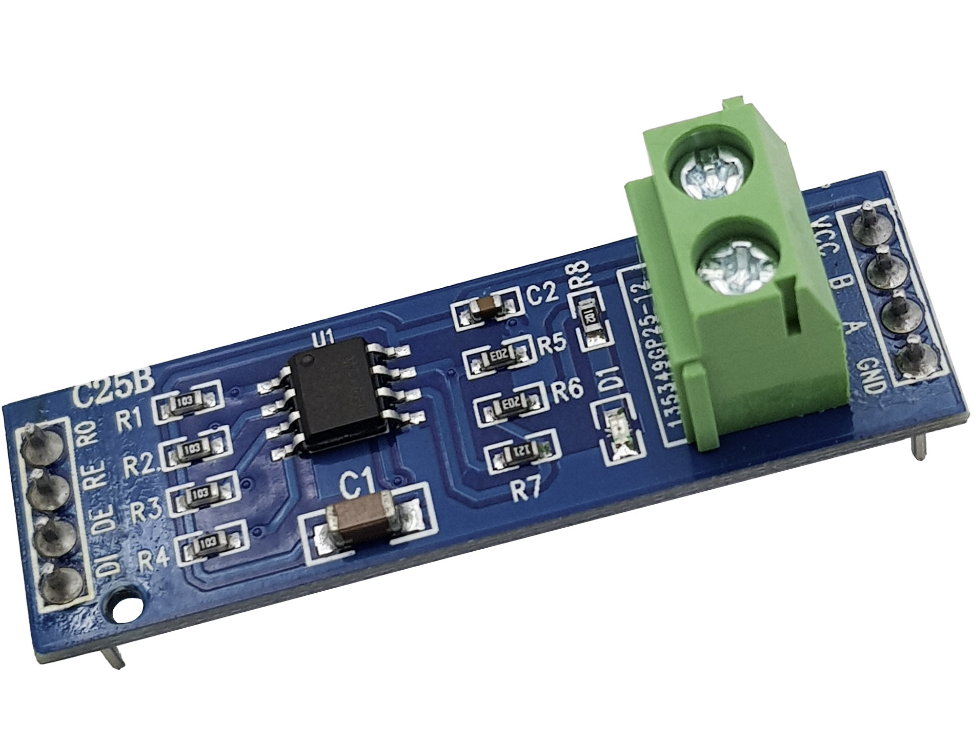
\includegraphics[scale=0.6]{Image/Content_1/Module.png}
	\caption{Module giao tiếp TTL RS485}
\end{figure}

Hệ thống được chạy và hiển thị thông số trên Thingsboard để dễ dàng tiếp cận đến người dùng

\begin{figure}[H]
	\centering
	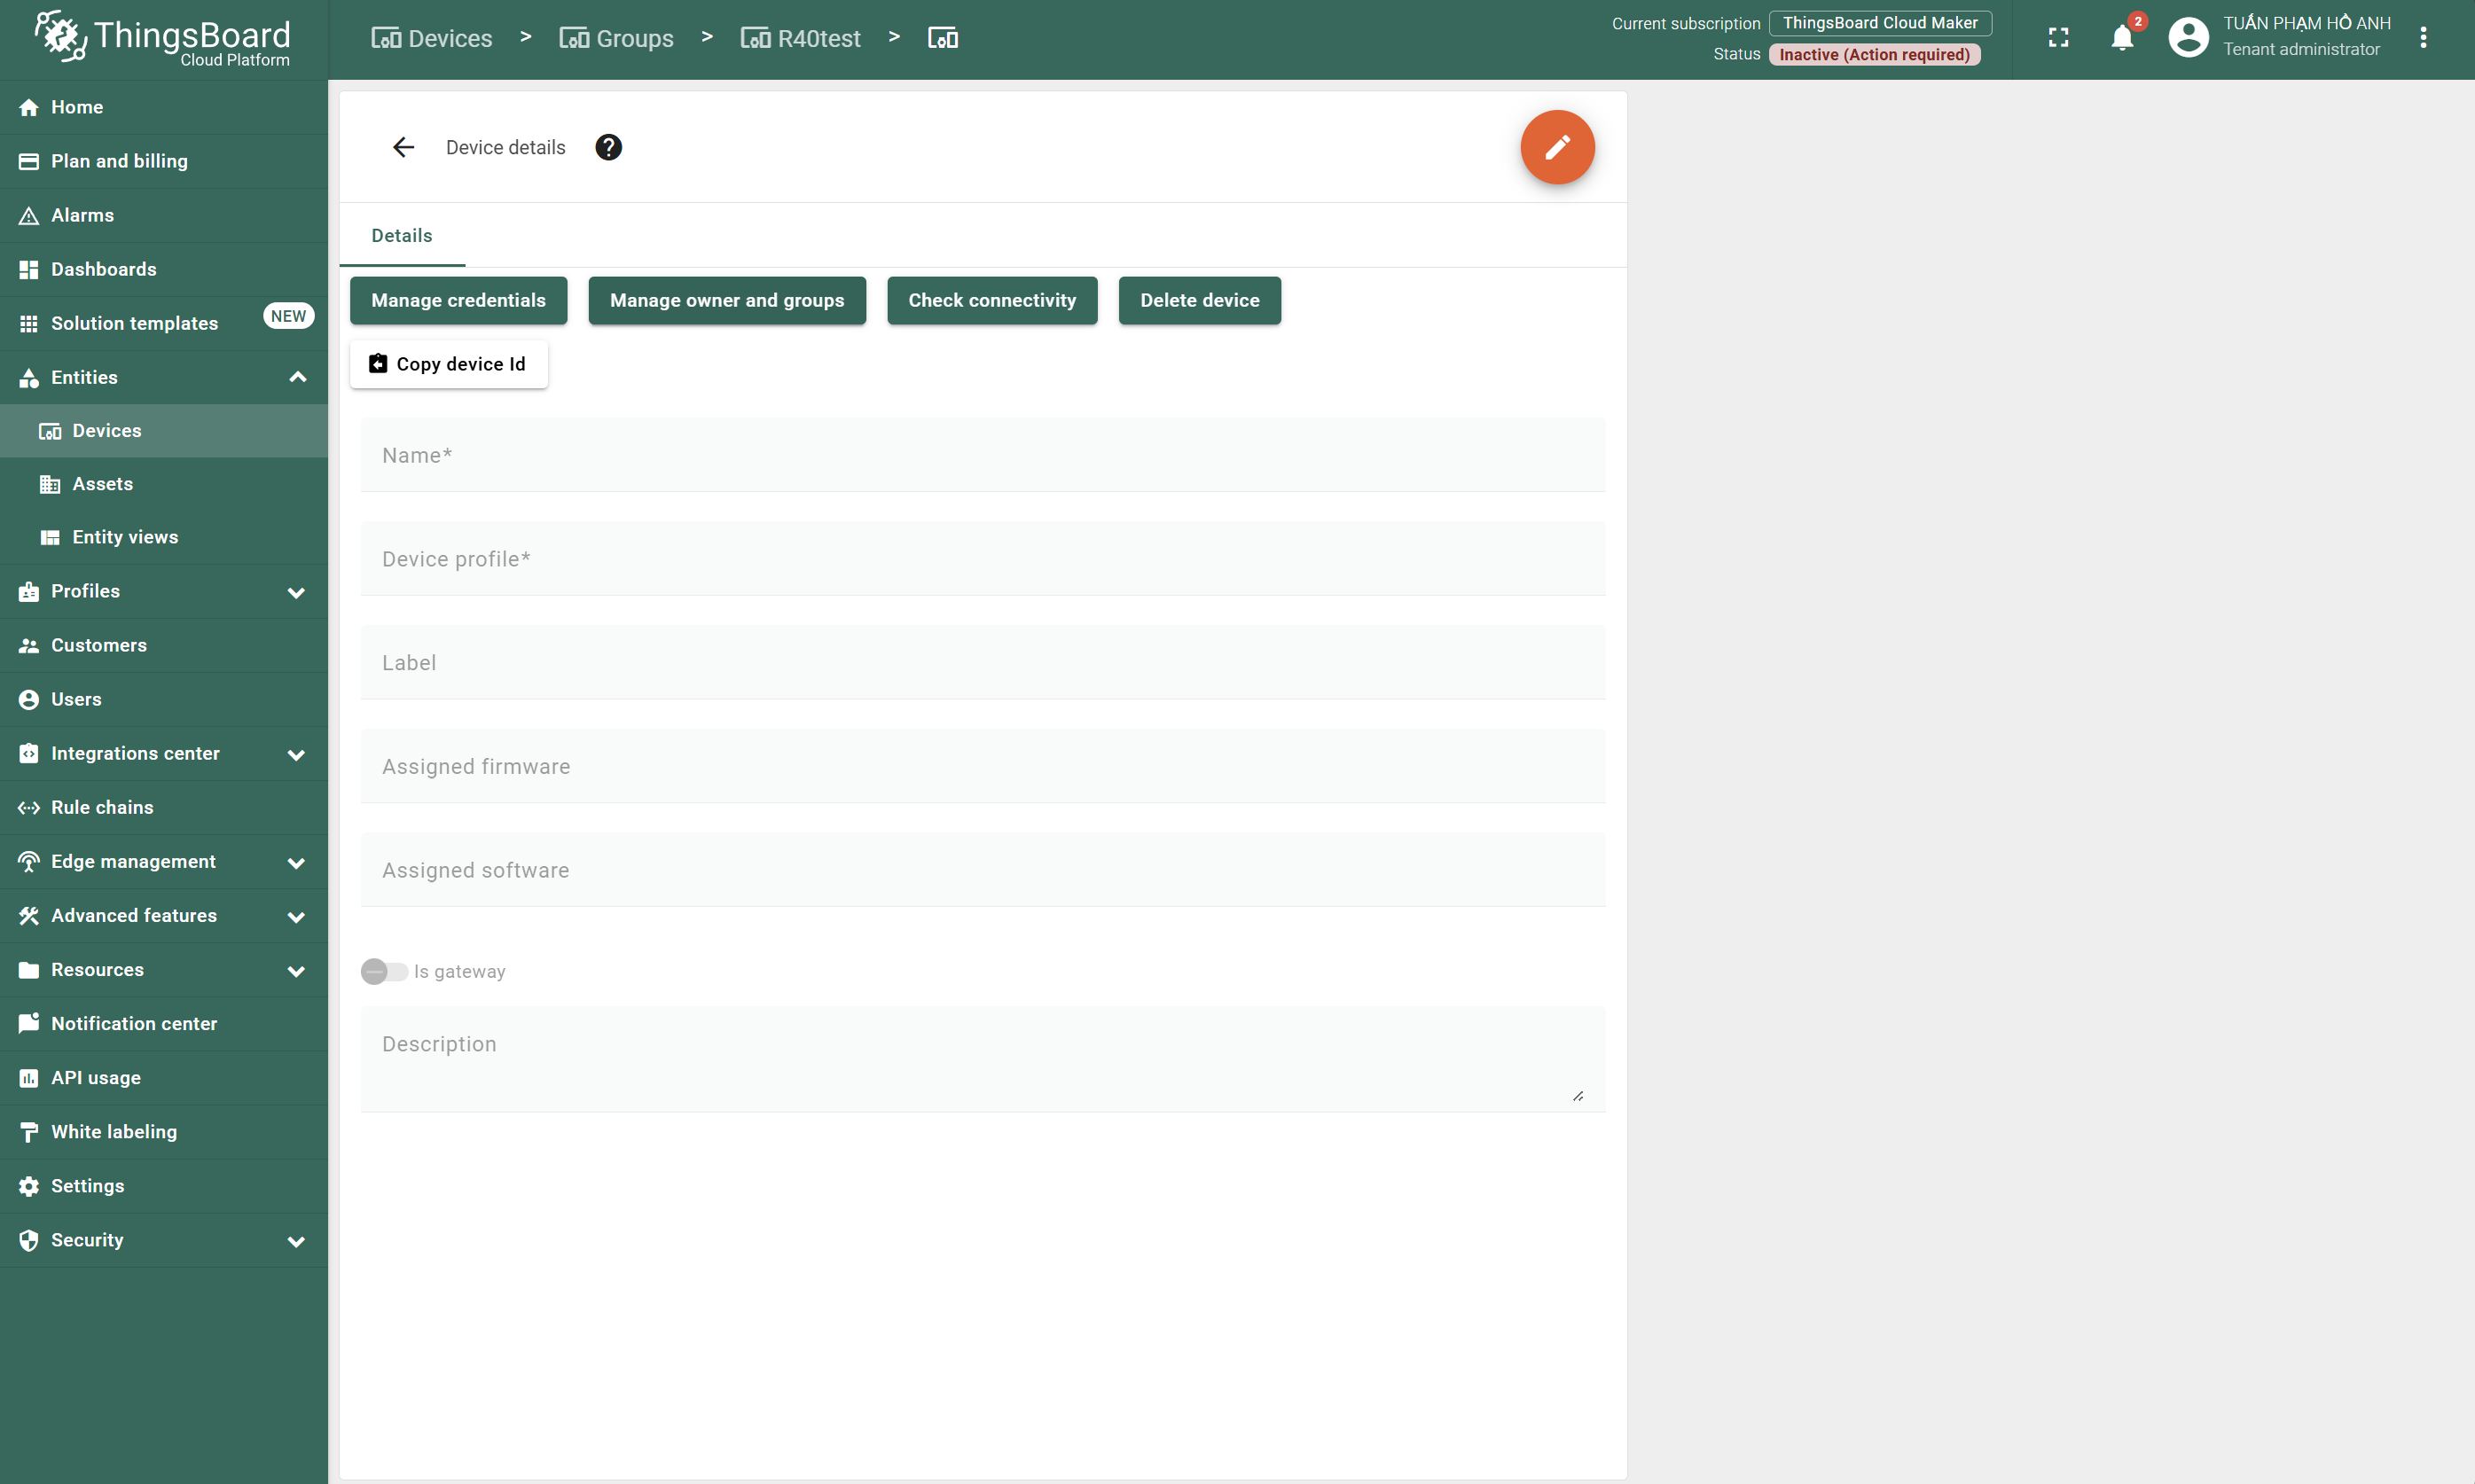
\includegraphics[scale=0.3]{Image/Content_1/Thingsboard.png}
	\caption{Nền tảng Thingsboard}
\end{figure}

Hệ thống được điều khiển và hoạt động trên vi điều khiển ESP32 được hỗ trợ kết nối wifi bằng SmartConfig, hoạt động kết nối wifi được thực hiện trên app EspTouch

\begin{figure}[H]
	\centering
	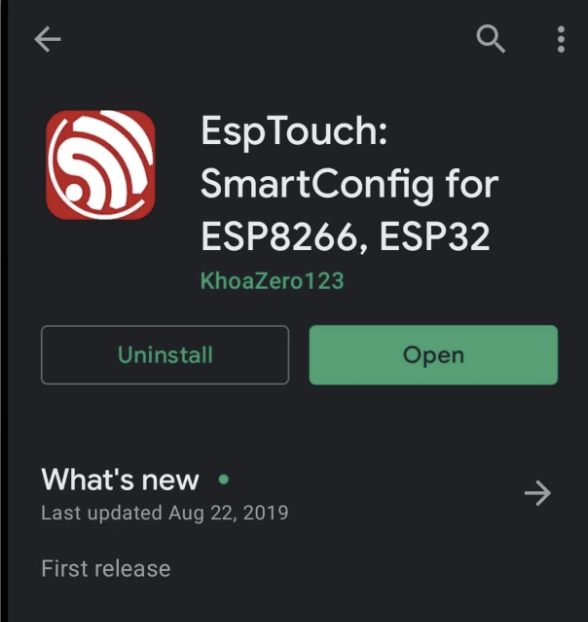
\includegraphics[scale=0.7]{Image/Content_1/Esptouch.png}
	\caption{App EspTouch trên điện thoại di động}
\end{figure}

\subsubsection*{4.3. Kiểm tra hoạt động của ADC trên hai dòng chip AVR và STM32}
\addcontentsline{toc}{subsection}{\numberline{} 4.3. KKiểm tra hoạt động của ADC trên hai dòng chip AVR và STM32}

- Kiểm tra hoạt động của ADC trên chip Atmega324PA:

\begin{figure}[H]
	\centering
	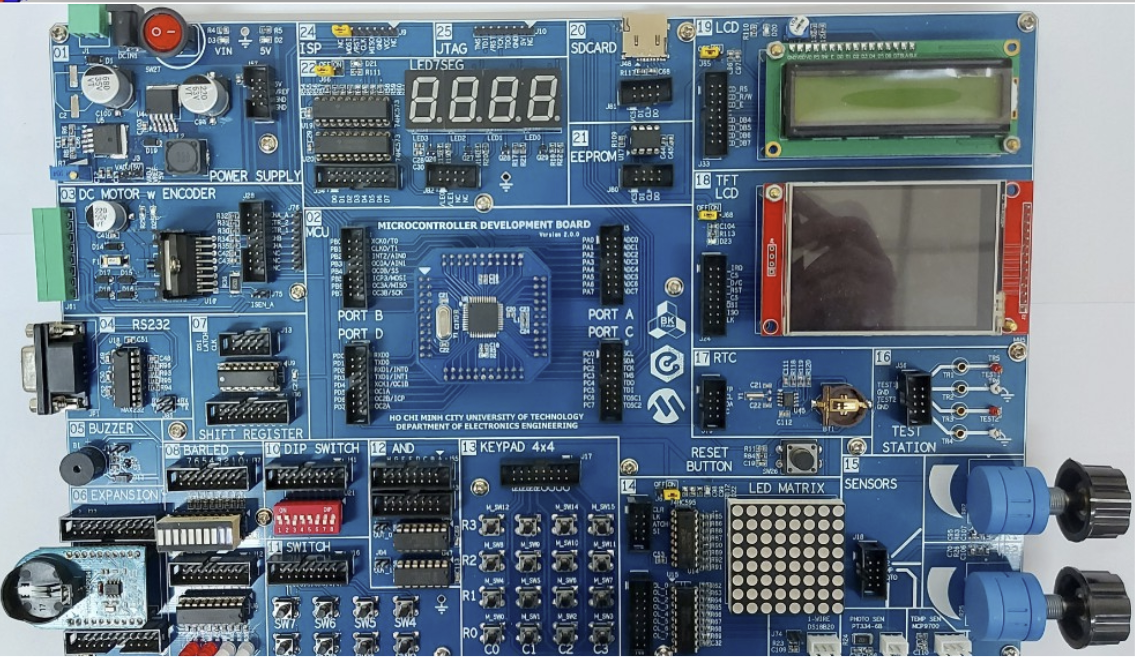
\includegraphics[scale=0.7]{Image/Content_1/ATmega.png}
	\caption{Kit vi xử lý Atmega324PA}
\end{figure}

Sử dụng đoạn code sau để đọc giá trị ADC ghi vào và lấy mẫu để xem xét tính tuyến tính:

\begin{figure}[H]
	\centering
	\includegraphics[scale=0.7]{Image/Content_1/CodeATmega.png}
	\caption{Code đọc ADC ATmega324PA}
\end{figure}

- Kiểm tra hoạt động của ADC trên chip STM32F030F4P6:

\begin{figure}[H]
	\centering
	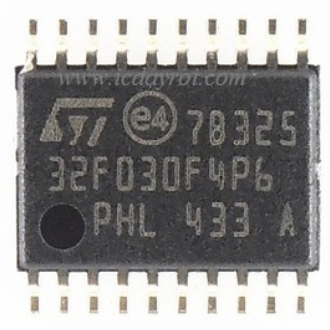
\includegraphics[scale=0.7]{Image/Content_1/STM32F0.png}
	\caption{STM32F030F4P6}
\end{figure}

Vẽ mạch ra chân và đọc ADC cho chip STM32F030F4P6

\begin{figure}[H]
	\centering
	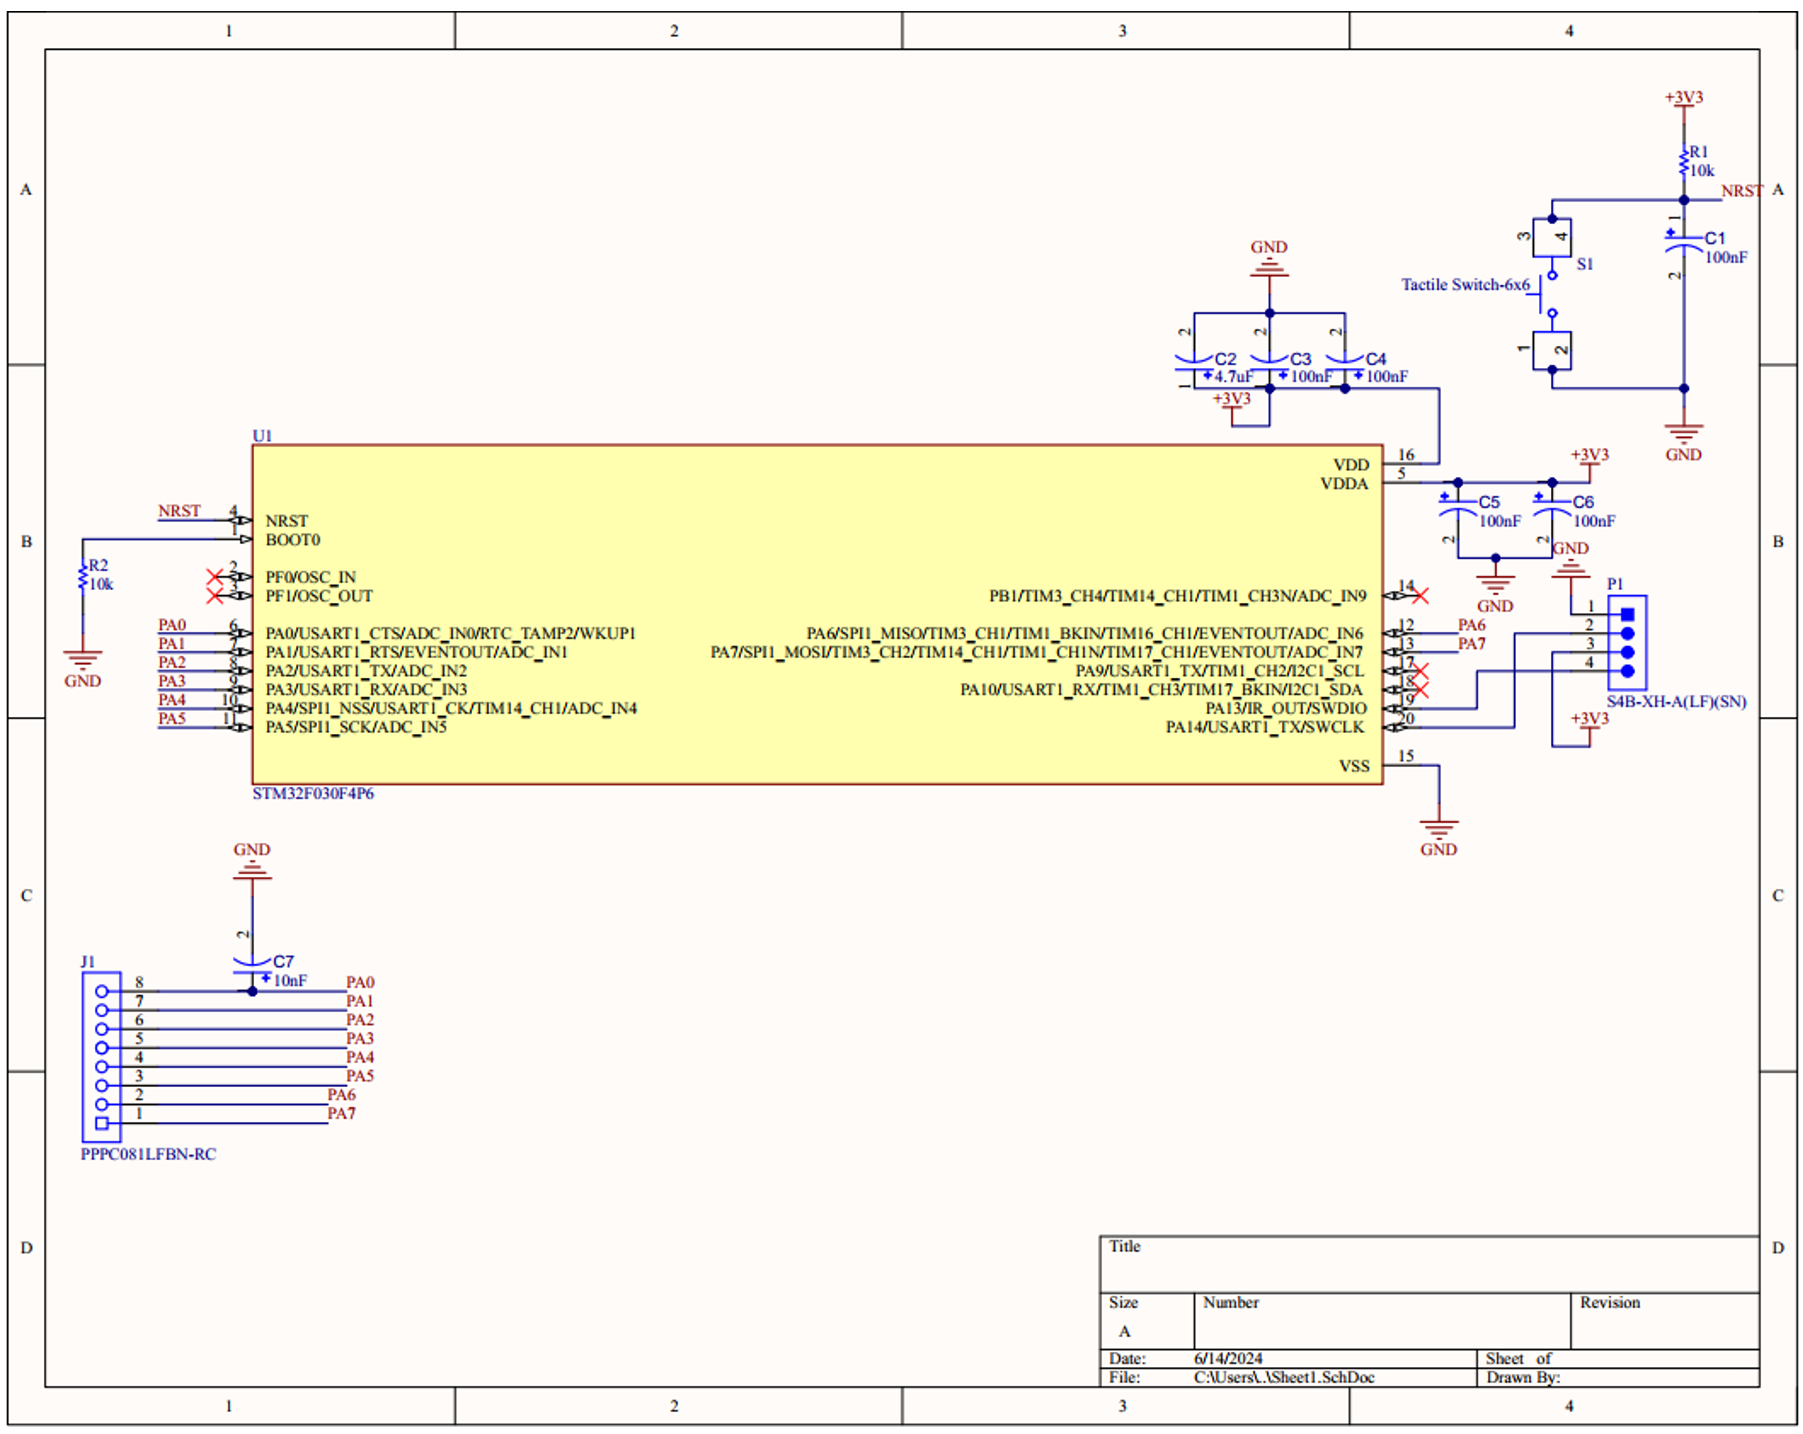
\includegraphics[scale=0.5]{Image/Content_1/Sche.png}
	\caption{Schematic mạch ra chân ADC cho STM32F030FF4P6}
\end{figure}

Cấu hình và code đọc giá trị ADC ghi vào và lấy mẫu để xem xét tính tuyến tính:

\begin{figure}[H]
	\centering
	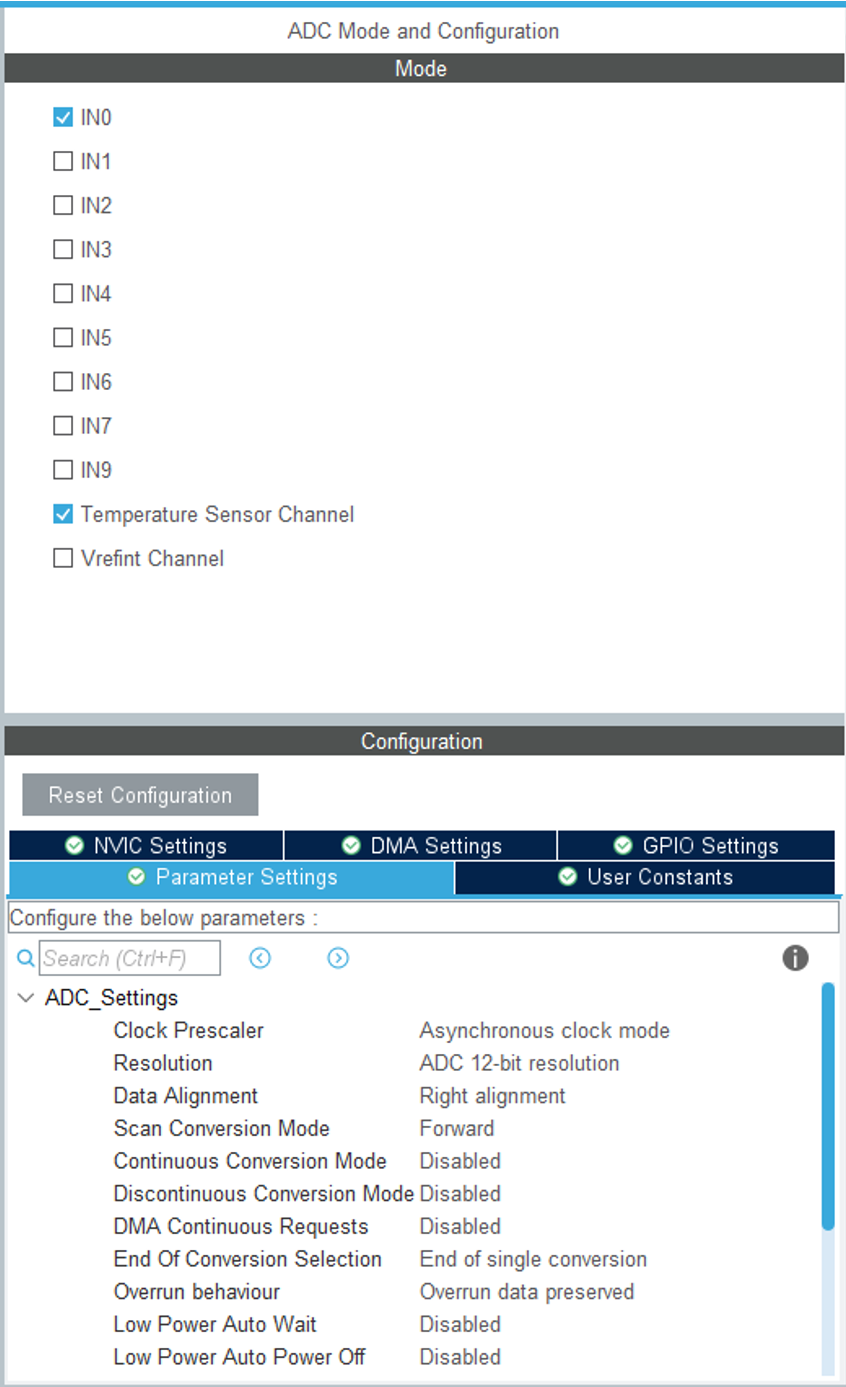
\includegraphics[scale=0.5]{Image/Content_1/ConfigADC.png}
	\caption{Thứ tự config ADC}
\end{figure}

\begin{figure}[H]
	\centering
	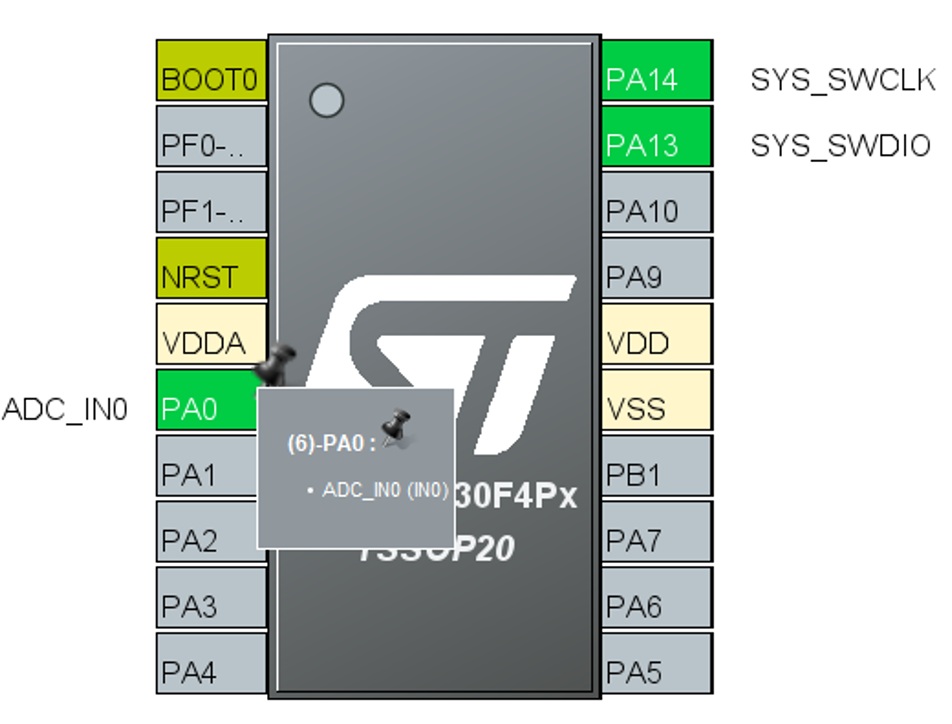
\includegraphics[scale=0.5]{Image/Content_1/PinoutADC.png}
	\caption{Set output ADC trên IOC}
\end{figure}

- Kiểm tra hoạt động của ADC trên chip STM32F411VET6 (Discovery):

\begin{figure}[H]
	\centering
	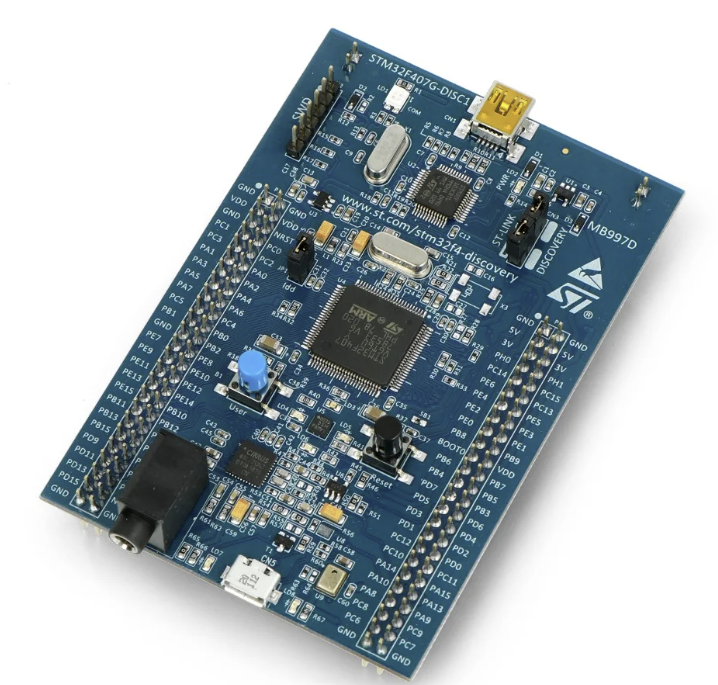
\includegraphics[scale=0.5]{Image/Content_1/STM32F4.png}
	\caption{STM32F411VET6}
\end{figure}

Cấu hình và code đọc giá trị ADC ghi vào và lấy mẫu để xem xét tính tuyến tính:

\begin{figure}[H]
	\centering
	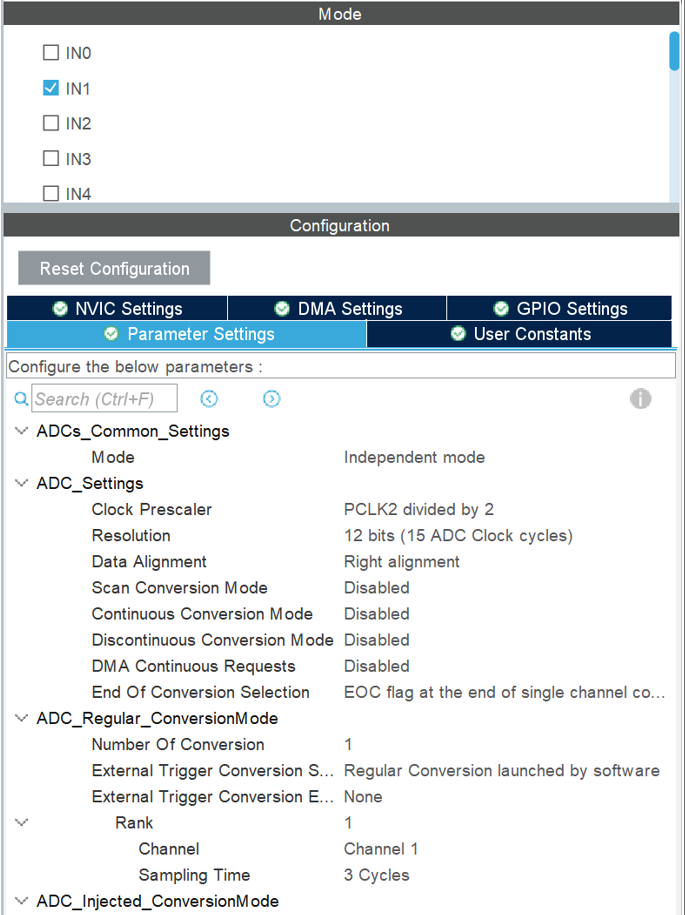
\includegraphics[scale=0.8]{Image/Content_1/ConfigF4.png}
	\caption{Cấu hình cho STM32F4}
\end{figure}

\begin{figure}[H]
	\centering
	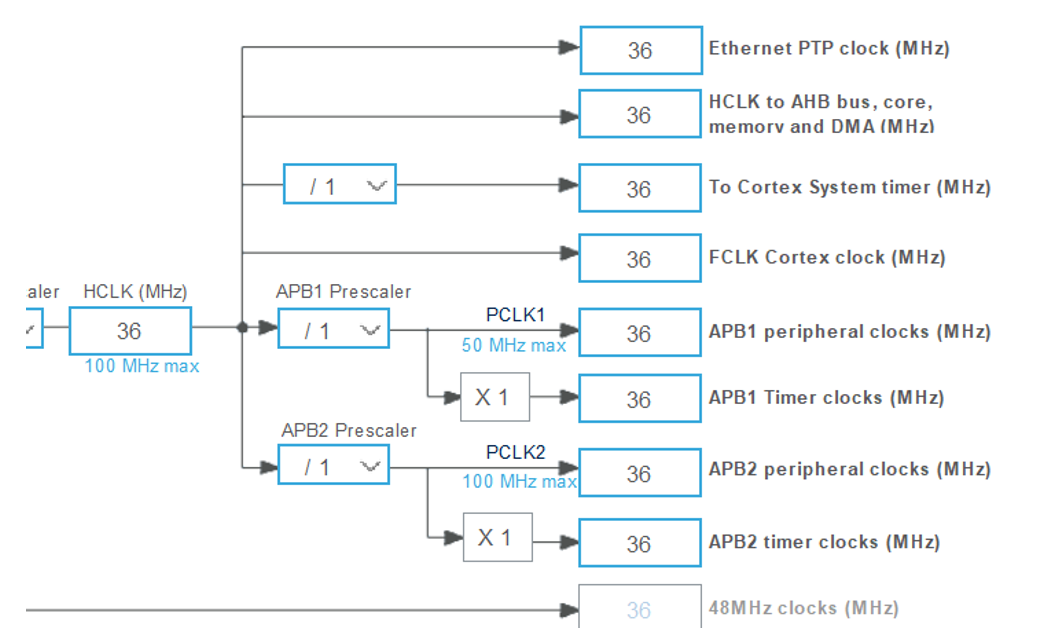
\includegraphics[scale=0.7]{Image/Content_1/ConfigClock.png}
	\caption{Cấu hình xung clock cho STM32F4}
\end{figure}

\begin{figure}[H]
	\centering
	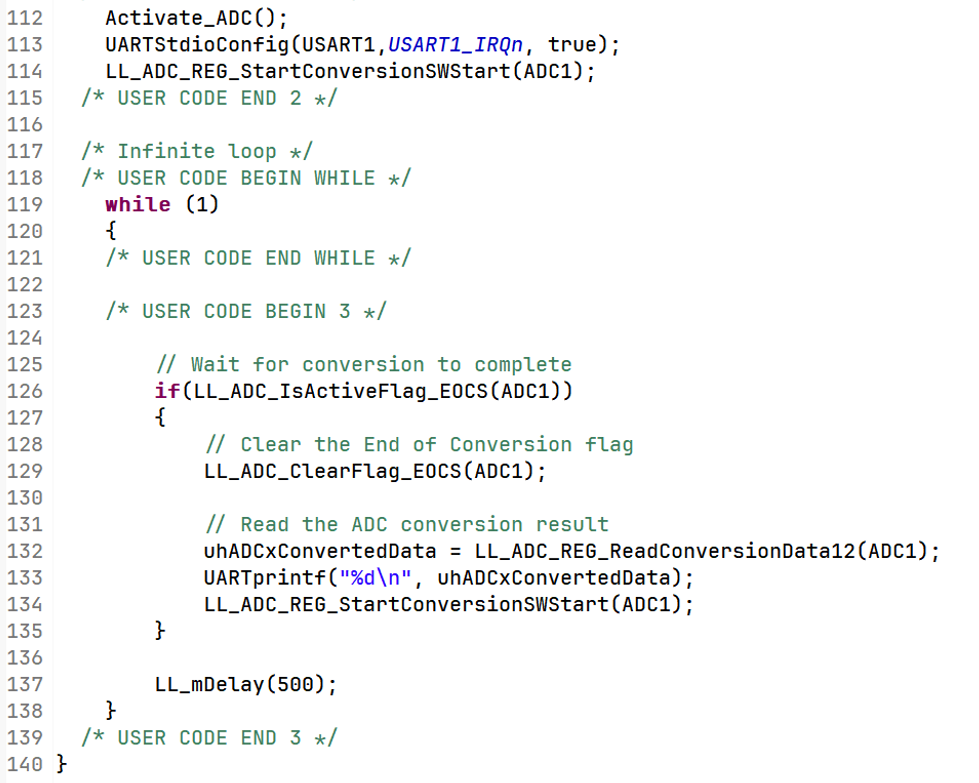
\includegraphics[scale=0.7]{Image/Content_1/CodeADCF4.png}
	\caption{Code đọc ADC cho STM32F4 bằng thư viện LL}
\end{figure}

\subsubsection*{4.4. Nghiên cứu và phát triển USB Mass Storage bằng ESP32 và STM32}
\addcontentsline{toc}{subsection}{\numberline{} 4.4. Nghiên cứu và phát triển USB Mass Strorage bằng ESP32 và STM32} 

\subsubsection*{4.4.1. Giới thiệu lý do sử dụng USB Mass Storage trên STM32 và ESP32}
\addcontentsline{toc}{subsection}{\numberline{} 4.4.1. Giới thiệu lý do sử dụng USB Mass Storage trên STM32 và ESP32} 

- STM32 và ESP32 đều là các vi điều khiển phổ biến trong các ứng dụng nhúng, nhưng bộ nhớ tích hợp thường bị hạn chế. Việc sử dụng USB Mass Storage cho phép mở rộng khả năng lưu trữ một cách dễ dàng mà không cần phải thêm các chip nhớ ngoài phức tạp. Điều này đặc biệt hữu ích khi cần lưu trữ dữ liệu lớn như log, hình ảnh, hoặc tệp nhị phân. \\
- USB Mass Storage là một tiêu chuẩn phổ biến, được hỗ trợ rộng rãi trên hầu hết các hệ điều hành. Điều này có nghĩa là các thiết bị sử dụng STM32 và ESP32 có thể dễ dàng kết nối và truyền dữ liệu với máy tính hoặc thiết bị khác mà không cần phần mềm đặc biệt. Tính năng plug-and-play này giúp việc phát triển và triển khai các giải pháp lưu trữ trở nên thuận tiện và hiệu quả hơn.\\
- Khi tích hợp USB Mass Storage vào dự án, bạn có thể tận dụng các thư viện và driver có sẵn như FatFs trên STM32 hoặc ESP32. Điều này không chỉ giúp tiết kiệm thời gian phát triển mà còn giảm bớt công sức viết code quản lý bộ nhớ phức tạp. Sự hỗ trợ tốt từ cộng đồng và các ví dụ có sẵn giúp các nhà phát triển dễ dàng tích hợp và tùy chỉnh theo nhu cầu của dự án.\\
- USB Mass Storage trên STM32 và ESP32 có thể được ứng dụng trong nhiều lĩnh vực khác nhau như thiết bị ghi dữ liệu (data logger), hệ thống nhúng thông minh, thiết bị IoT, và các ứng dụng cần lưu trữ dữ liệu liên tục hoặc lớn. Khả năng này làm cho STM32 và ESP32 trở thành lựa chọn lý tưởng cho các dự án cần giải pháp lưu trữ tin cậy và linh hoạt. \\
- STM32 và ESP32 đều cung cấp hiệu suất xử lý cao và khả năng quản lý USB một cách hiệu quả. Khi kết hợp với USB Mass Storage, chúng có thể cung cấp tốc độ truyền dữ liệu nhanh, đáp ứng được các ứng dụng đòi hỏi sự ổn định và tốc độ. Đồng thời, cả STM32 và ESP32 đều có giá thành phải chăng, giúp giảm thiểu chi phí trong quá trình phát triển sản phẩm.\\

\subsubsection*{4.4.2. Cấu hình USB Mass Storage trên STM32F746NGH6}
\addcontentsline{toc}{subsection}{\numberline{} 4.4.2. Cấu hình USB Mass Storage trên STM32F746NGH6} 

Cấu hình USB hoạt động ở mode device với class USB Mass Strorage:

\begin{figure}[H]
	\centering
	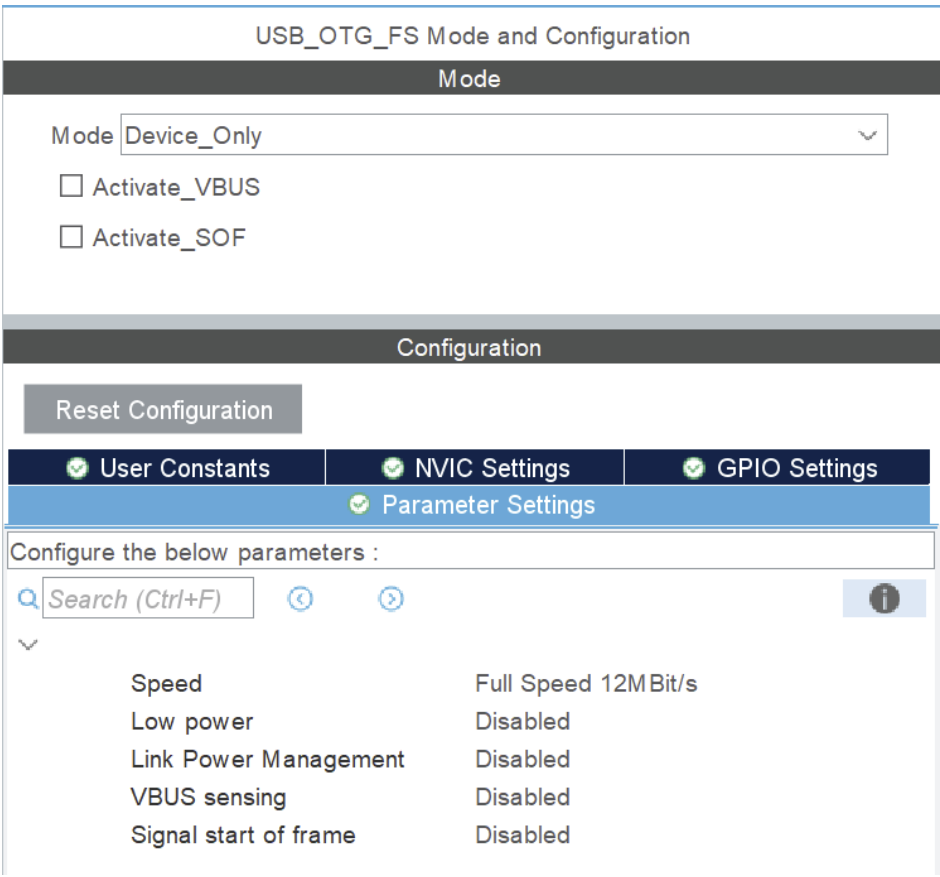
\includegraphics[scale=0.6]{Image/Content_1/USB_Config.png}
	\caption{Cấu hình USB Mass Storage cho STM32F7}
\end{figure}

\begin{figure}[H]
	\centering
	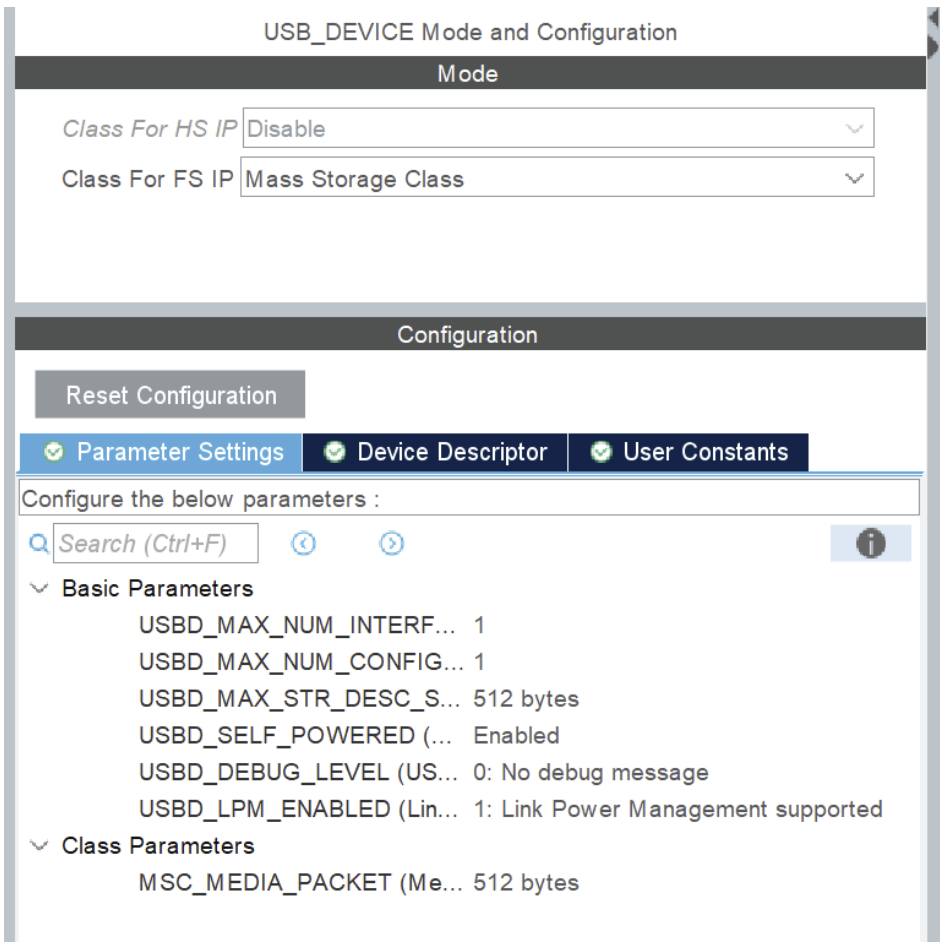
\includegraphics[scale=0.6]{Image/Content_1/USB_Config_1.png}
	\caption{Cấu hình USB Mass Storage cho STM32F7}
\end{figure}

- Cấu hình xung clock USB hoạt động:

\begin{figure}[H]
	\centering
	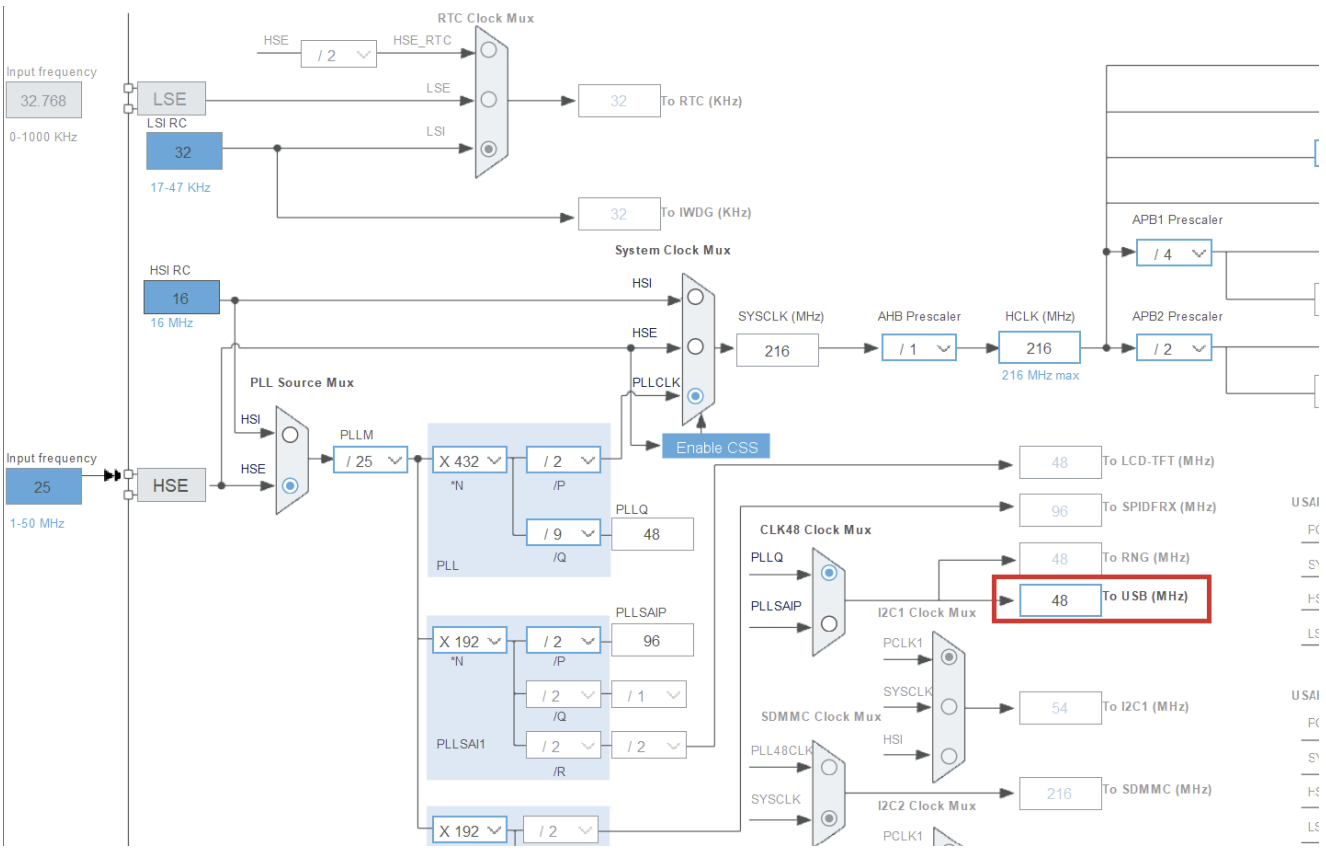
\includegraphics[scale=0.6]{Image/Content_1/ClockUSB_Config.png}
	\caption{Cấu hình xung clock USB}
\end{figure}

\subsubsection*{4.4.3. Cấu hình USB Mass Storage trên ESP32S3}
\addcontentsline{toc}{subsection}{\numberline{} 4.4.3. Cấu hình USB Mass Storage trên ESP32S3} 

- Đối với ESP32 chỉ có dòng chip ESP32-S3 mới hỗ trợ USB Mass Strorage.\\
- Cấu hình USB hoạt động ở mode device với class USB Mass Strorage, đồng thòi sử
dụng SD-CARD giao tiếp qua giao thức SDMMC để làm bộ nhớ lưu trữ:\\

\begin{lstlisting}[language = c]
	ESP_ERROR_CHECK ( storage_init_sdmmc (& sd_card ) ) ;
	/* First way to register the callback . This is while
	initializing the storage . */
	const tinyusb_msc_sdmmc_config_t config_sdmmc =
	{
		. card = & sd_card ,
		. callback_mount_changed =
		storage_mount_changed_cb ,
		. mount_config . max_files = 5 ,
	};
	ESP_ERROR_CHECK ( tinyusb_msc_storage_init_sdmmc (&
	config_sdmmc ) ) ;
	ESP_ERROR_CHECK ( tinyusb_msc_register_callback (
	TINYUSB_MSC_EVENT_MOUNT_CHANGED ,
	storage_mount_changed_cb ) ) ;
	const tinyusb_config_t tusb_cfg =
	{
		. device_descriptor = & descriptor_config ,
		. string_descriptor = string_desc_arr ,
		. string_descriptor_count =
		sizeof ( string_desc_arr ) / sizeof (
		string_desc_arr [0]) ,
		. external_phy = false ,
		. configuration_descriptor =
		desc_configuration ,
	};
	ESP_ERROR_CHECK ( tinyusb_driver_install (& tusb_cfg ) ) ;
\end{lstlisting}


\subsubsection*{4.5. Viết tài liệu tham khảo về FATFs và cách sử dụng FATFs}
\addcontentsline{toc}{subsection}{\numberline{} 4.5. Nghiên cứu và phát triển USB Mass Strorage bằng ESP32 và STM32} 

\subsubsection*{4.5.1. Giới thiệu về FATFs}
\addcontentsline{toc}{subsection}{\numberline{} 4.5.1. Giới thiệu về FATFs} 

- FATFs là một thư viện được sử dụng để quản lý hệ thống file, bao gồm việc định
dạng, tạo, đọc, ghi, và xóa các tệp và thư mục trên một vùng nhớ nhất định, như
thẻ SD hoặc bộ nhớ flash. Nó hỗ trợ các hệ thống file phổ biến như FAT12, FAT16,
FAT32, và exFAT, cho phép các hệ thống nhúng có thể tương tác với các thiết bị lưu
trữ ngoài giống như cách mà một máy tính tiêu chuẩn hoạt động với các hệ thống
file này.\\

- FATFs cung cấp các API để thao tác với tệp và thư mục, giúp quản lý dữ liệu trên
các thiết bị lưu trữ dễ dàng và hiệu quả trong các ứng dụng nhúng.\\

- Fast File System (FFS) được thiết kế với mục tiêu cải thiện hiệu suất và quản lý dữ
liệu hiệu quả hơn so với các hệ thống tập tin trước đó. Để đạt được điều này, FFS
đã giới thiệu một số khái niệm và cấu trúc mới, đồng thời cải tiến các yếu tố cốt lõi
của hệ thống tập tin.\\

\begin{figure}[H]
	\centering
	\includegraphics[scale=0.7]{Image/Content_1/FATFs_arc.png}
	\caption{Cấu hình xung clock USB}
\end{figure}

\begin{figure}[H]
	\centering
	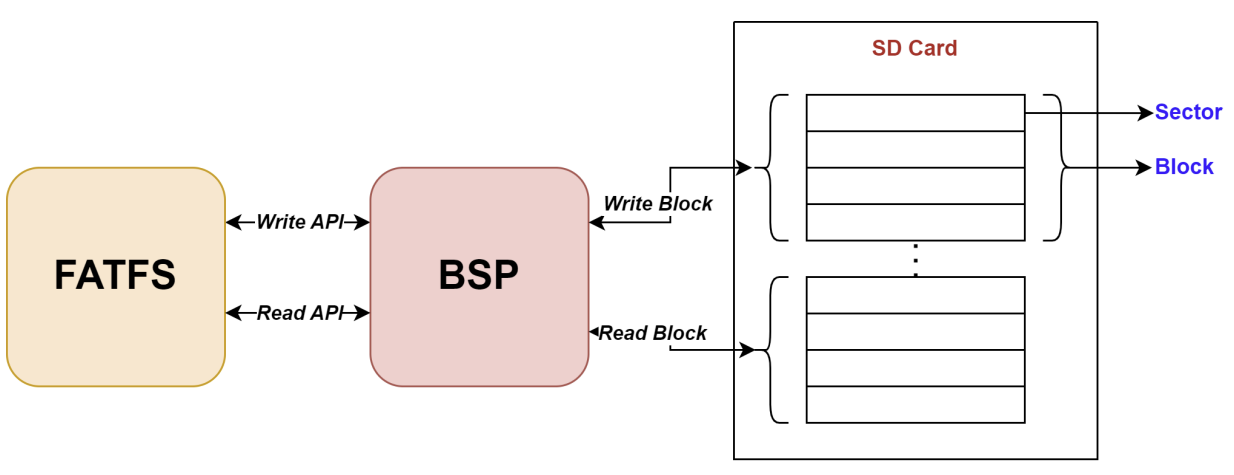
\includegraphics[scale=0.7]{Image/Content_1/API_FATFs.png}
	\caption{Sơ đồ API FATFs hoạt động trên STM32}
\end{figure}

- Các API của FATFs hoạt động dựa trên hai lớp thư viện chính: FATFs và BSP
(Board Support Package):\\
FATFs: Đây là lớp thư viện chịu trách nhiệm quản lý hệ thống file, bao gồm các
chức năng như tạo, đọc, ghi, và xóa tệp và thư mục. FATFs cung cấp các API
để ứng dụng có thể tương tác với hệ thống file trên một thiết bị lưu trữ như thẻ
SD hoặc bộ nhớ flash.\\
BSP (Board Support Package): Lớp này đóng vai trò giao tiếp trực tiếp với phần
cứng, cụ thể là SD-CARD. BSP xử lý việc truyền tải dữ liệu giữa vi điều khiển
và SD-CARD thông qua các giao thức phần cứng như:\\
Trong kiến trúc này, lớp BSP sẽ xử lý các tương tác cấp thấp với SD-CARD, bao
gồm việc gửi và nhận dữ liệu thông qua các giao thức như SPI, SDIO hoặc SDMMC.
Lớp FATFs sử dụng các dịch vụ từ BSP để thực hiện các thao tác hệ thống file, như đọc và ghi tệp. Sự phân chia này giúp tách biệt logic hệ thống file với chi tiết phần
cứng, làm cho mã nguồn dễ bảo trì và mở rộng hơn.\\

\subsubsection*{4.5.2. Tích hợp thư viện FATFs vào một dự án sử dụng chip STM32}
\addcontentsline{toc}{subsection}{\numberline{} 4.5.2. Tích hợp thư viện FATFs vào một dự án sử dụng chip STM32}

FATFs là một thư viện mã nguồn mở, được phát triển và bảo trì bởi cộng đồng,
với các bản sửa lỗi và cập nhật thường xuyên để cải thiện hiệu suất và độ tin cậy.
Vì lý do này, khi sử dụng FATFs trong các dự án nhúng, bạn nên tải và sử dụng
thư viện trực tiếp từ nhà phát hành chính thức thay vì dựa vào mã tự động tạo ra
bởi STM32CubeIDE. STM32CubeIDE có thể tích hợp các phiên bản của FATFs,
nhưng đôi khi những phiên bản này có thể không được cập nhật kịp thời với các
bản sửa lỗi mới nhất. Điều này có thể dẫn đến việc sử dụng các phiên bản FATFs
chưa được tối ưu hóa hoặc có lỗi chưa được khắc phục, gây ra những vấn đề không
mong muốn trong quá trình phát triển. Do đó, để đảm bảo độ tin cậy và tối ưu cho
dự án, việc sử dụng phiên bản FATFs mới nhất từ nhà phát hành chính thức là một
lựa chọn an toàn và hiệu quả hơn.

Thư viện FATFs có rất nhiều chức năng, và để tối ưu hóa hiệu suất và dung lượng
bộ nhớ sử dụng, việc bật hoặc tắt các tính năng cụ thể theo đúng mục đích sử dụng
của dự án là cần thiết.

\newpage
\section*{PHẦN II: KẾT QUẢ THỰC TẬP}
\addcontentsline{toc}{section}{\numberline{} PHẦN II: KẾT QUẢ THỰC TẬP}

\subsection*{1. Phát triển hệ thống giám sát cường độ sáng}
\addcontentsline{toc}{subsection}{\numberline{} 1. Phát triển hệ thống giám sát cường độ sáng}

- Dashboard được thiết kế trên ThingsBoard.

 \begin{figure}[H]
 	\centering
 	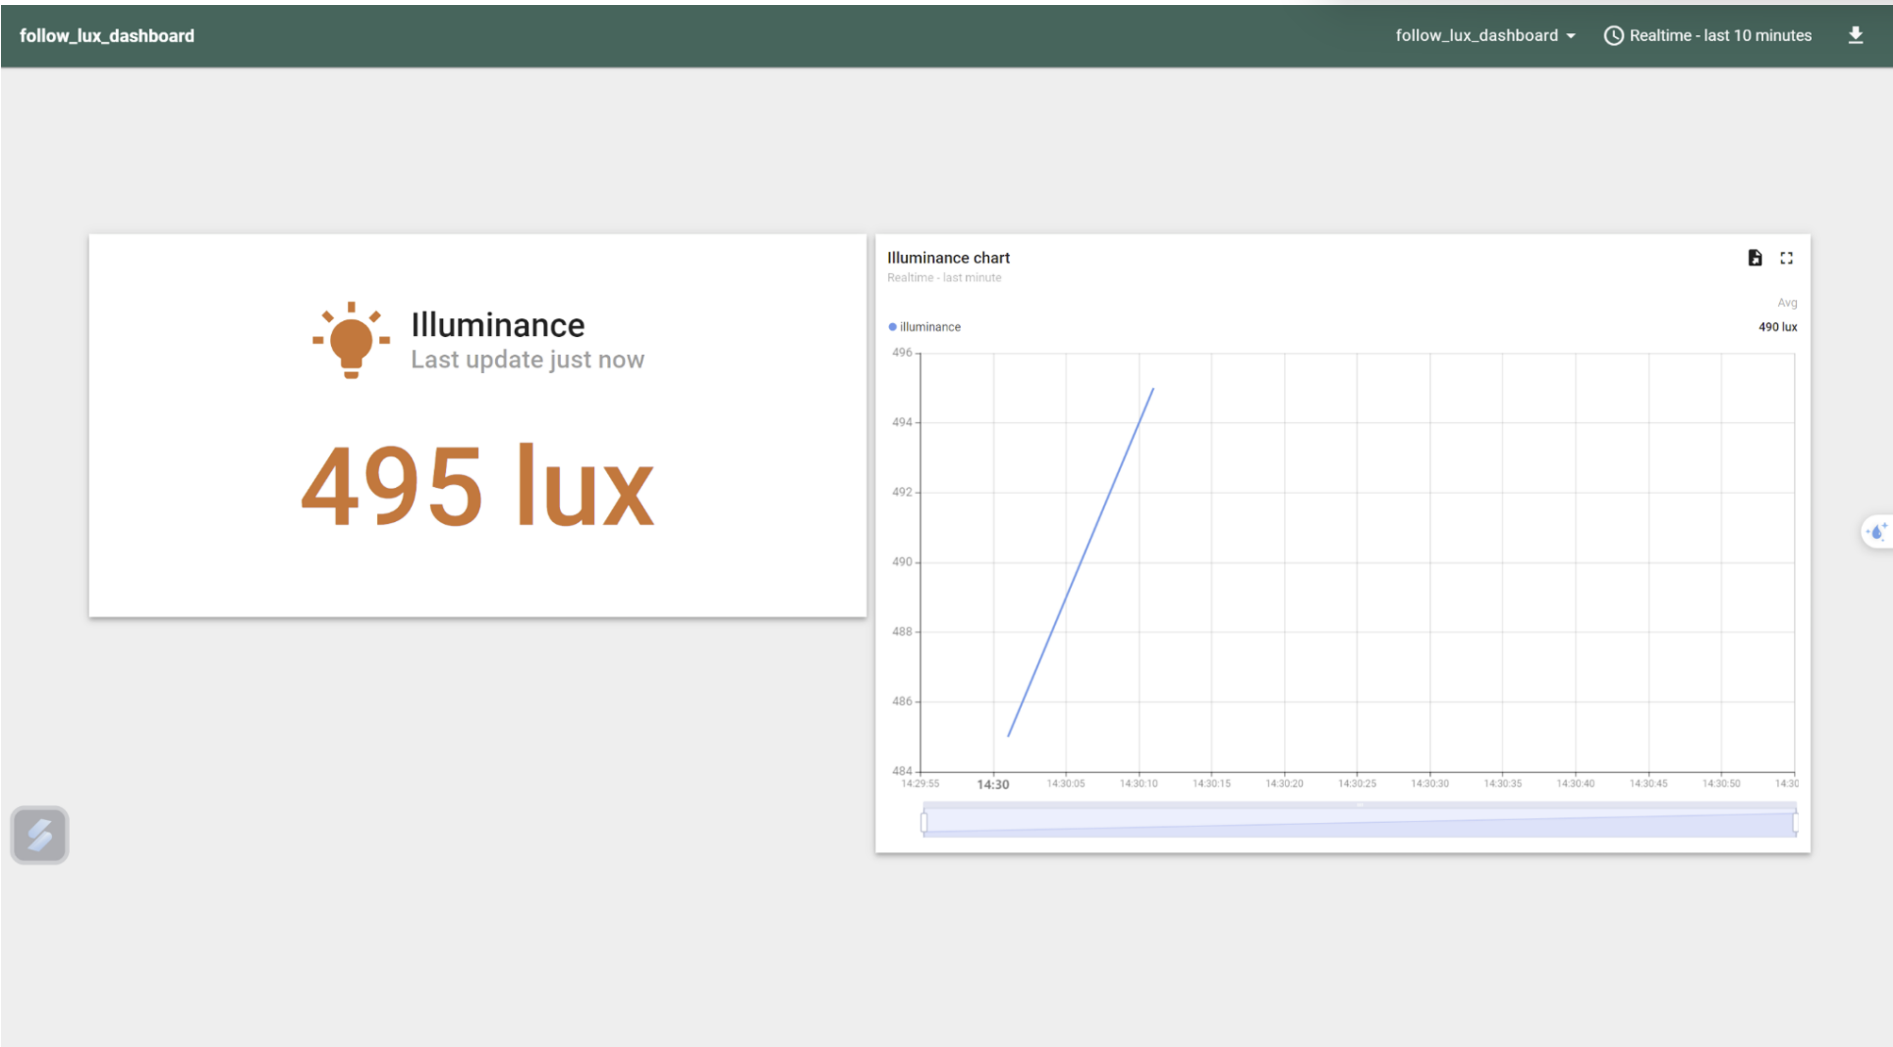
\includegraphics[scale=0.5]{Image/Content_1/Dashboard.png}
 	\caption{Dashboard}
 \end{figure}

\subsection*{2. Kiểm tra hoạt động ADC trên hai dòng chip AVR và STM32}
\addcontentsline{toc}{subsection}{\numberline{} 2. Kiểm tra hoạt động ADC trên hai dòng chip AVR và STM32}

Mạch đo ADC cho chip STM32F030F4P6:

 \begin{figure}[H]
	\centering
	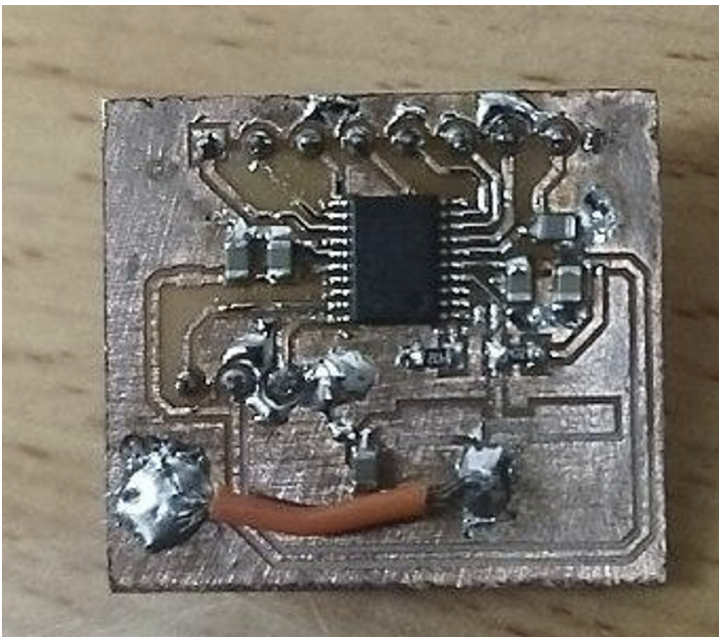
\includegraphics[scale=0.5]{Image/Content_1/ADC_F0.png}
	\caption{Dashboard}
\end{figure}

Kết quả sau khi do đạc cho ba dòng chip:\\
– STM32F411VET6:

 \begin{figure}[H]
	\centering
	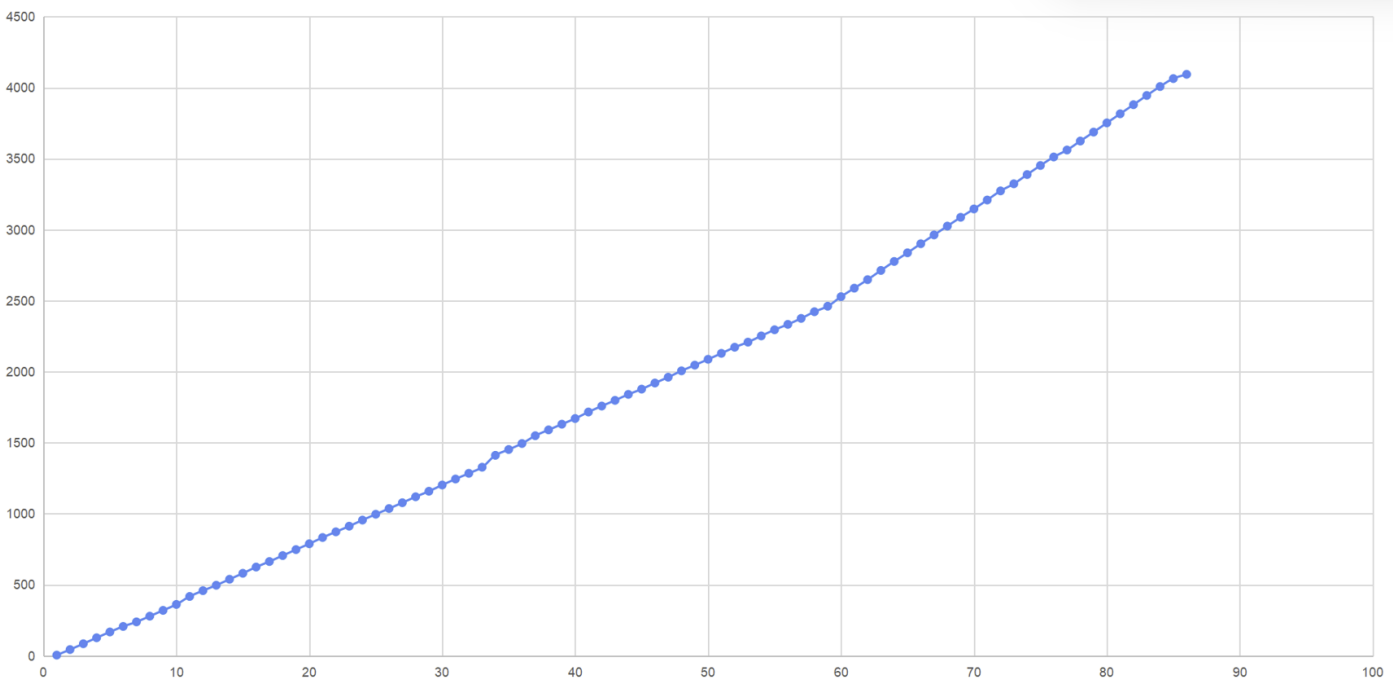
\includegraphics[scale=0.5]{Image/Content_1/ADC_F4.png}
	\caption{Kết quả đo ADC chip STM32F411VET6}
\end{figure}

- ATMEGA324PA:
 \begin{figure}[H]
	\centering
	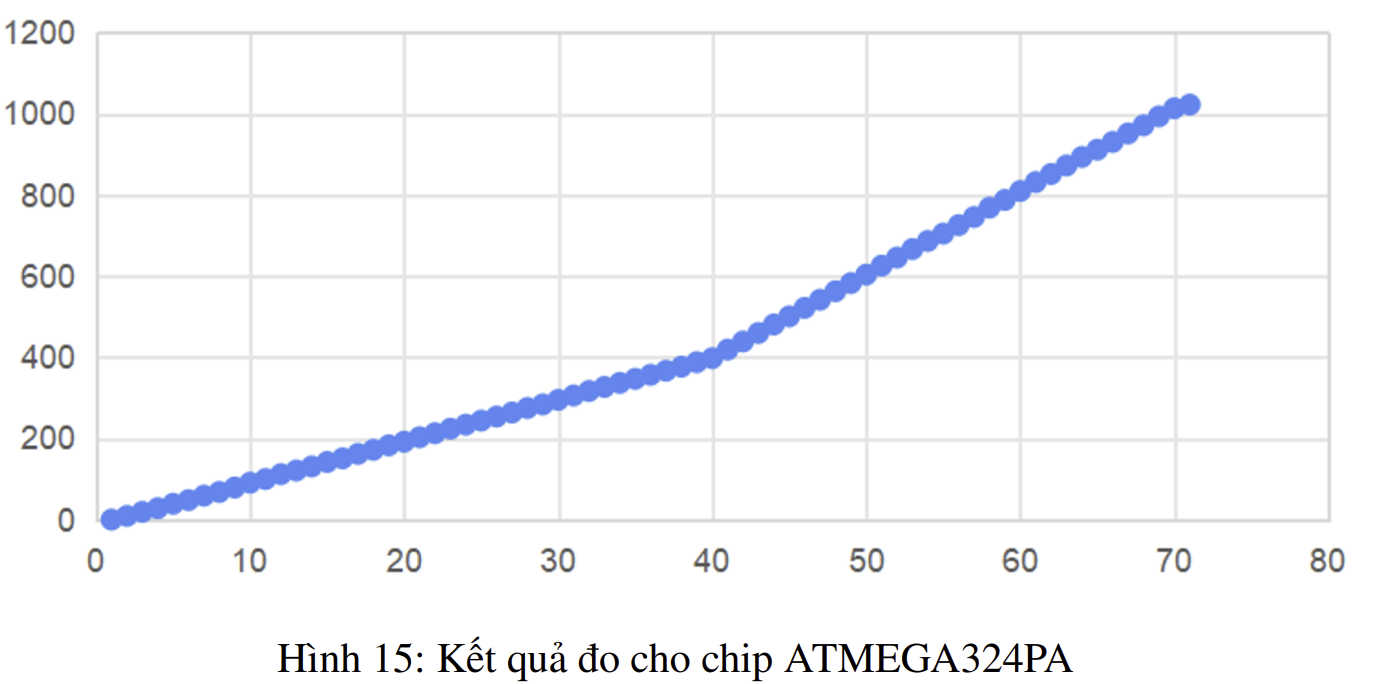
\includegraphics[scale=0.5]{Image/Content_1/ADC_AVR.png}
	\caption{Kết quả đo ADC chip ATMEGA324PA}
\end{figure}

- STM32F030F4P6:
 \begin{figure}[H]
	\centering
	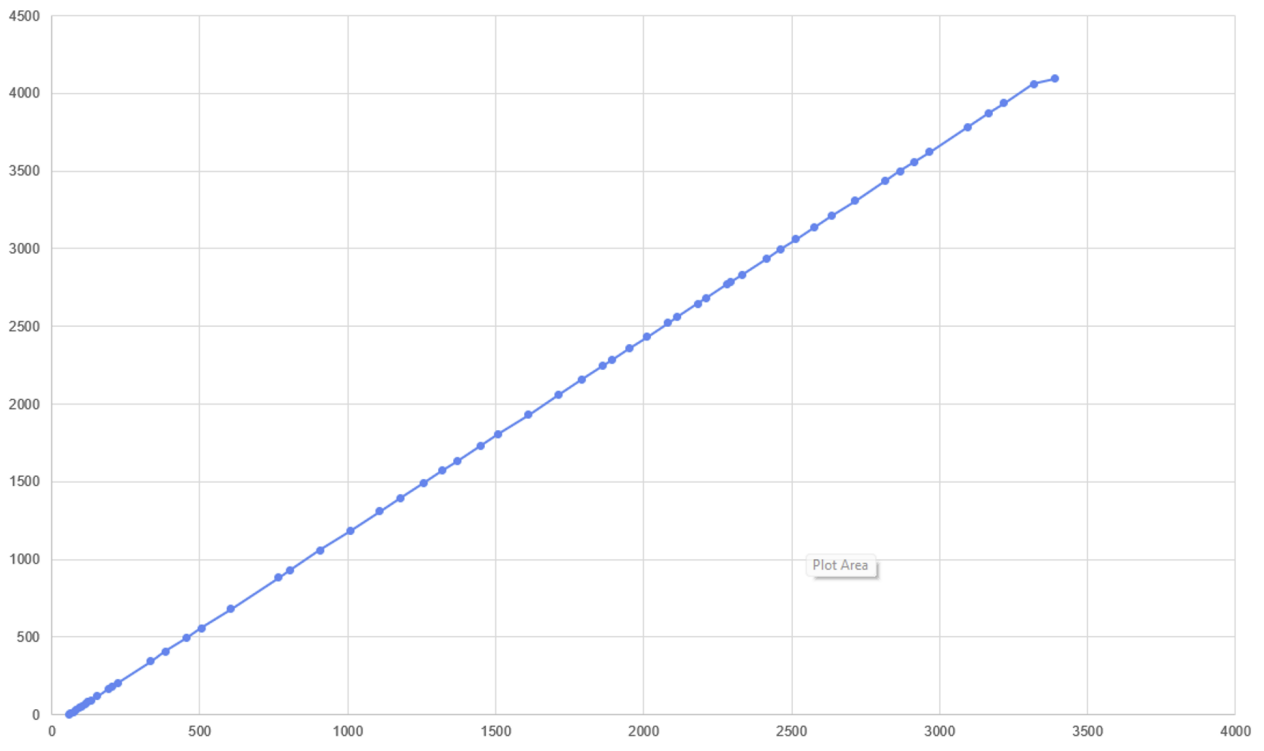
\includegraphics[scale=0.5]{Image/Content_1/ADC_F00.png}
	\caption{Kết quả đo ADC chip STM32F030F4P6}
\end{figure}

Từ các đồ thị thu về sau khi kiểm tra, ta có thể kết luận dòng chip STM32F030F4P6
hoạt động với độ tuyến tính cao nhất từ đó đó có thể đưa ra con số chính xác nhất.

\newpage
\section*{PHẦN III: TỔNG KẾT THỰC TẬP}
\addcontentsline{toc}{section}{\numberline{} PHẦN III: TỔNG KẾT THỰC TẬP}

\subsection*{1. Kinh nghiệm, kiến thức học được sau khi thực tập}
\addcontentsline{toc}{subsection}{\numberline{} 1. Kinh nghiệm, kiến thức học được sau khi thực tập}

- Kỳ thực tập đã giúp em có cái nhìn cận cảnh về ngành nghề mình đang theo đuổi,
một cái nhìn trực quan về sự khó khăn, vất vả trong môi trường làm việc thực tế. Tất
cả mọi khâu, mọi quá trình, mọi công tác đều được thực hiện với một sự cẩn trọng,
tỉ mỉ, chính xác cao và tập trung cao độ tuyệt đổi. Bởi vì người kỹ sư điện biết rằng,
chỉ cần một sai lầm dù là nhỏ nhất, thì sự cố có thể xảy ra bất cứ lúc nào và ở đâu.\\
- Về phía bản thân mình, chặng đường tương lai ở phía trước vẫn còn rất dài và chông
gai. Để trở thành một kỹ sư giỏi, có ích cho xã hội sau này, em còn phải cố gắng rất
nhiều nữa. Kỳ thực tập vừa rồi đã giúp em phần nào thêm yêu thích công việc mà
em đang theo đuổi, và cũng cho em thấy rằng ngành nghề này cũng đầy ắp những
khó khăn, và chính vì lý do đó, em cần phải cố gắng phấn đấu hơn nữa trong việc
học tập để có thể thành công trong tương lai. Bên cạnh những kiến thức, kỹ năng
học được trong quá trình thực tập, bản thân còn có cơ hội được làm quen với văn
hóa làm việc có trách nhiệm, tác phong chuyên nghiệp cùng với tình thần tự giác
cao của các anh trong phòng lab.\\

\subsection*{2. Cảm nghĩ sau thực tập}
\addcontentsline{toc}{subsection}{\numberline{} 2. Cảm nghĩ sau thực tập}

- Sau thời gian thực tập, được trải nghiệm một đề tài thực tế, em đã học hỏi được rất
nhiều điều từ Thầy và các anh, như tác phong làm việc, cách thức mà mọi người
phối hợp, giúp đỡ nhau trong công việc. Từ đó, em hiểu hơn về vai trò, trách nhiệm
của bản thân trong các công việc chung trong một nhóm. Đồng thời thông qua kỳ
thực tập này, em cũng được nâng cao khả năng tự học, tự tìm hiểu khi phải tiếp xúc
với một dự án, kiến thức mới.\\

\clearpage